\section{XACML use comparison}\label{sec:xacml-use}

\begin{figure}[ht]
    \centering
    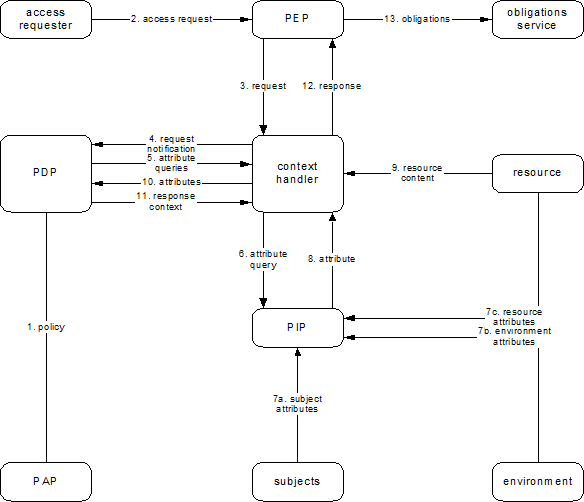
\includegraphics[width=\textwidth]{xacml-architecture}
    \caption{\acrshort{xacml} data flow diagram. Taken from~\cite{OASISStandard2013EXtensible3.0}.}
    \label{fig:xacml-architecture}
\end{figure}

\begin{sidewaysfigure}[ht]
    \centering
    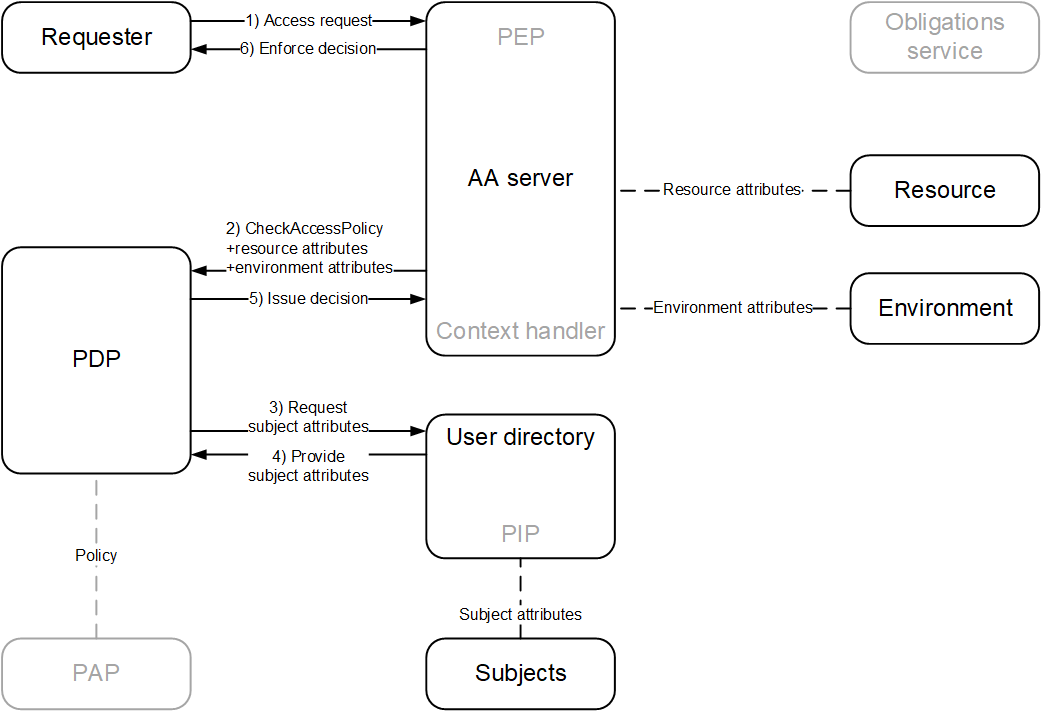
\includegraphics[width=.85\textwidth]{xacml-use}
    \caption{Data flow diagram of the proposed system. The parts in grey are not discussed in the report. In step two, the \acrshort{aaserver} supplies additional context information (resource and environment attributes) in its \texttt{CheckAccessPolicy} request. Furthermore, the \acrshort{aaserver} enforces the policy decision by issuing the access token if the policy evaluation is \textit{Allow access}, or by denying to issue the access token and returning an error message, if the evaluation decision is \textit{Deny access}.}
    \label{fig:xacml-use}
\end{sidewaysfigure}